\section{Bayesian Statistics}
Bayesian statistics is based on \dfref{def:bayesian_statistics}, which follows the definition of subjective probability (\dfref{def:subjective_probability}) and the treating the parameters as realizations of a random variable (\axref{ax:parameter_variable}). The Bayesian framework originally come from the work of \citet{Bayes:63} and \citet{laplace_thorie_1812} with much of the modern discussions and formalism created later by \citet{Finetti1937LaP,Jeffreys1940} and \citet{Savage1954}.\newline
In the Bayesian paradigm, it is assumed that Natures decisions can be captured by a statistical model with parameters that are modeled as realizations of random variables. This means that the probability $p(S=s|X=x,D,I)$ in equation \EQref{eq:decision_rule3} depend on the parameters $w_1,\dots w_n$ of the statistical model. Introducing the shorthand notation $W=w_1\dots W=w_n \rightarrow w$, $dw_1\dots dw_n \rightarrow dw$ and $X=x \rightarrow x$, then
\begin{equation}
	\begin{split}
		p(s|x,D,I) &= \int dw p(w,s|x,D,I)\\
		& = \int dw p(s|w,x,D,I)p(w|x,D,I)
	\end{split}
	\label{eq:hest1}
\end{equation}
\begin{example}
	Writing out the shorthand notation
	\begin{equation}
		\begin{split}
			p(W=w_1,\dots,W= w_n,S = s|X = x,D,I)&\rightarrow p(w,s|x,D,I),\\
			dw_1\dots dw_n &\rightarrow dw.\\
		\end{split}
	\end{equation}
\end{example}

To evaluate $p(w|D,I)$ a combination of the chain rule (\thref{theorem:chain_rule}), Bayes' theorem (\thref{theorem:bayes_theorem}) and marginalization (\thref{theorem:law_of_total_probability}) can be employed viz
\begin{equation}
	\begin{split}
		p(w|x,D,I) &= p(w|D,I)\\
		&= \frac{p(D_s|w,D_x,I)p(w|I)}{p(D_s|D_x,I)},
	\end{split}
	\label{eq:pa2}
\end{equation}
where $D_s= \{S=s_1\dots S=s_n\}$, $D_x = \{X=x_1,\dots X=x_n\}$ and $p(D_s|D_x,I)$ can be expanded via marginalization and \axref{ax:observation_relevance} has been used for the first and second equality.

\begin{axiom}[Relevance of Observations]
	\label{ax:observation_relevance}
	The Robot's observations are relevant for estimating Nature's model only when they map to known actions of Nature.
\end{axiom}

$p(w|I)$ is the Robot's prior belief about $w$. $p(D_s|w,D_x,I)$ is the likelihood of the past observations of Nature's actions, and $p(w|D,I)$ called the posterior distribution represent the belief of the Robot after seeing data. The prior distribution depends on parameters that must be specified and cannot be learned from data since it reflects the Robot's belief before observing data. These parameters are included in the background information, $I$. From \EQref{eq:pa2}, it is evident that, given the relevant probability distributions are specified, the probability of a parameter taking a specific value follows deductively from probability theory. The subjectivity arises from the assignment and specification of probability distributions which depend on the background information.



\subsection{Bayesian Regression}
\label{chp:regression}
Regression involves the Robot building a model, $f: \Omega_W\times \Omega_X\mapsto\mathbb{R}$, with associated parameters $w\in \Omega_W$, that estimates Nature's actions $S$ based on observed data $X$. Note that the output of $f$ is $\mathbb{R}$ implying that $S$ is assumed continuos. The model $f$ acts as a proxy for the Robot in that it on behalf of the Robot estimates the action of Nature given an input. Hence, in providing an estimate, the model must make a choice, similar to the Robot and thus the Robot must pick a cost function for the model. In this study, the quadratic cost function from \dfref{def:quadratic_cost} will be considered to review the subject. From \thref{theorem:expectation_decision_rule} the best action for the Robot can be written
\begin{equation}
	U^*(x) = \int ds s p(s|x,D,I)
	\label{eq:q1}
\end{equation}
Assuming the actions of Nature follow a normal distribution with the function $f$ as mean and an unknown precision, $\xi\in \Omega_W$
\begin{equation}
	p(s|x,w,\xi,I)=\sqrt{\frac{\xi}{2\pi}} e^{-\frac{\xi}{2}(f(w,x)-s)^2}.
	\label{f_dist}
\end{equation}
Using \EQref{f_dist} and marginalizing over $\xi,w$
\begin{equation}
	\begin{split}
		p(s|x,D,I) &= \int p(s,w,\xi|x,D,I) dw d\xi\\
		& = \int p(s|x,w,\xi,D,I)  p(w,\xi|x,D,I)dw d\xi\\
		& = \int p(s|x,w,\xi,I)  p(w,\xi|D,I)dw d\xi,\\
	\end{split}
	\label{eq:q2}
\end{equation}
where it has been used that $p(s|w,\xi,x,D,I) = p(s|w,\xi,x,I)$ since by definition $f$ produce a $1-1$ map of the input $x$ (\EQref{f_dist}) and $p(w,\xi|x,D,I) = p(w,\xi|D,I)$ from \axref{ax:observation_relevance}. Using \EQref{eq:q2} in \EQref{eq:q1}\footnote{Note that a function of a random variable is itself a random variable, so $f$ is a random variable.}
\begin{equation}
	\begin{split}
		U^*(x) & = \int f(w,x)  p(w,\xi|D,I) dw d\xi,\\
		& = \mathbb{E}[f|x,D,I]
	\end{split}
	\label{eq:q3}
\end{equation}	
where it has been used that
\begin{equation}
	\begin{split}
		\mathbb{E}[S|x,w,\xi,I] &= \int s p(s|x,w,\xi,I) dy\\
		&= f(w,x)
	\end{split}
\end{equation}
according to \EQref{f_dist}. Using Bayes theorem (\thref{theorem:bayes_theorem})
\begin{equation}
	p(w,\xi|D,I) = \frac{p(D_s|D_x,w,\xi,I)p(w,\xi|D_x,I)}{p(D_s|D_x,I)}
	\label{eq:bayes2}
\end{equation}
where from marginalization (\thref{theorem:law_of_total_probability})
\begin{equation}
	p(D_s|D_x,I) = \int p(D_s|D_x,w,\xi,I)p(w,\xi|D_x,I) dw d\xi.
\end{equation}
Assuming the past actions of Nature are independent and identically distributed, the likelihood can be written (using equation \EQref{f_dist})
\begin{equation}
	p(D_s|D_x,w,\xi,I) = \bigg(\frac{\xi}{2\pi}\bigg)^\frac{n}{2}\prod_{i=1}^n e^{-\frac{\xi}{2}(f(w,x_i)-s_i)^2}
	\label{reg:likelihood}
\end{equation}
From the chain rule (see \thref{theorem:chain_rule}) and \thref{ax:observation_relevance}
\begin{equation}
	p(w,\xi|D_x,I) = p(w|\xi,I)p(\xi|I).
\end{equation}
Assuming the distributions of the $w$'s are i) independent of $\xi$ and ii) normally distributed\footnote{The normally distributed prior is closely related to weight decay~\citep{Plaut1986}, a principle conventionally used in frequentist statistics to avoid the issue of overfitting.} with zero mean and a precision described by a hyperparameter, $\lambda$. 	 
\begin{equation}
	\begin{split}
		p(w|\xi,I) & = p(w|I)\\
		& = \int p(w|\lambda,I)p(\lambda|I)d\lambda
	\end{split}
	\label{eq:prior1}
\end{equation}
The precision is constructed as a wide gamma distribution\index{Gamma distribution} so as to approximate an objective prior
\begin{equation}
	p(w|\lambda,I)p(\lambda|I)
	= \prod_{q=1}^{\tilde{n}} \frac{\lambda_q^\frac{n_q}{2}}{(2\pi)^\frac{n_q}{2}}e^{-\frac{\lambda_q}{2}\sum_{l=1}^{n_q}w_l^2}\frac{\beta_q^{\alpha_q}}{\Gamma(\alpha_q)}\lambda_q^{\alpha_q-1}e^{-\beta_q \lambda_q}
	\label{eq:prior}
\end{equation}
where $\alpha_q,\beta_q$ are prior parameters (a part of the background information) and $\tilde{n}$ is the number of hyper parameters. In the completely general case $\tilde{n}$ would equal the number of parameters $w$, such that each parameter has an independent precision. In practice, the Robot may consider assigning some parameters the same precision, e.g. for parameters in the same layer in a neural network. Since $p(\xi|I)$ is analogous to $p(\lambda|I)$ -- in that both are prior distributions for precision parameters -- $p(\xi|I)$ is assumed to be a wide gamma distribution, then
\begin{equation}
	\begin{split}
		p(\xi|I) & = \text{Ga}(\xi|\tilde{\alpha},\tilde{\beta})\\
		& =\frac{\tilde{\beta}^{\tilde{\alpha}}}{\Gamma(\tilde{\alpha})}\xi^{\tilde{\alpha}-1}e^{-\tilde{\beta} \xi}.
	\end{split}
	\label{p7}
\end{equation}
At this point equation \EQref{eq:q1} is fully specified (the parameters $\alpha,\beta,\tilde{\alpha},\tilde{\beta}$ and the functional form of $f(w,x)$ are assumed specified as part of the background information) and can be approximated by obtaining samples from $p(w,\xi,\lambda|D,I)$ via HMC~\citep{Hammersley1964,Duane:1987de,Neal:1996,Neal2012} (see \appref{app:HMC} for a review of HMC). The centerpiece in the HMC algorithm is the Hamiltonian defined viz~\citep{Neal:1996,Neal2012}
\begin{equation}
	H \equiv  \sum_{q=1}^{\tilde{n}}\sum_{l=1}^{n_q}\frac{p_{l}^2}{2m_{l}}-\ln[p(w,\xi,\lambda|D,I)]+const,
	\label{eqh}
\end{equation}
where 
\begin{equation}
	p(w,\xi|D,I) = \int d\lambda p(w,\xi,\lambda|D,I).
	\label{eq:ss}
\end{equation}
Besides its function in the HMC algorithm, the Hamiltonian represent the details of the Bayesian model well and should be a familiar sight for people used to the more commonly applied frequentist formalism\index{Frequentist statistics} (since, in this case, it is in form similar to a cost function comprised of a sum of squared errors, weight decay on the coefficients and further penalty terms~\citep{hastie_09,murphy2013machine,Goodfellow2016}). Using \EQref{eq:bayes2}-\EQref{eq:ss} yields
\begin{equation}
	\begin{split}
		H&=\sum_{q=1}^{\tilde{n}}\sum_{l=1}^{n_q}\frac{p_{l}^2}{2m_{l}}+\frac{n}{2}[\ln(2\pi)-\ln(\xi)] +\frac{\xi}{2}\sum_{i=1}^{n}(f(w,x_i)-s_i)^2\\
		&\quad+\sum_{q=1}^{\tilde{n}}\bigg(\ln(\Gamma(\alpha_q))-\alpha_q\ln(\beta_q)+(1-\alpha_q)\ln(\lambda_q)+\beta_q\lambda_q\\
		&\qquad\qquad+\frac{n_q}{2}(\ln(2\pi)-\ln(\lambda_q))+\frac{\lambda_q}{2}\sum_{l=1}^{n_q}w_l^2\bigg)\\
		&\quad+\ln(\Gamma(\tilde{\alpha}))-\tilde{\alpha}\ln(\tilde{\beta})+(1-\tilde{\alpha})\ln(\xi)+\tilde{\beta}\xi+const.
	\end{split}
	\label{eqh2}
\end{equation}
\begin{example}
	\index{Example: HMC Hamiltonian variable change}
	Let $\xi \equiv e^\zeta$, such that $\zeta\in [-\infty,\infty]$ maps to $\xi\in[0,\infty]$ and $\xi$ is ensured to be positive definite regardless of the value of $\zeta$. Using the differential $d\xi =  \xi d\zeta$ in \EQref{eq:q3} means $p(\theta,\xi,\lambda|D,I)$ is multiplied with $\xi$. Hence, when taking $-\ln(p(\theta,\xi,\lambda|D,I))$ according to \EQref{eqh}, a $-\ln(\xi)$ is added to the Hamiltonian. In practice this means
	\begin{equation}
		(1-\tilde{\alpha})\ln(\xi)\in H\Rightarrow -\tilde{\alpha}\ln(\xi).
	\end{equation} 	
\end{example}



\begin{example}
	Suppose there is a game between a Robot and Nature in which the Robot objective is to guess the position of the Robot. The Robot is given measurements of its velocity and acceleration, at any time step and must formulate a belief about its position. Nature decides the true position of the Robot and will penalize the Robot according to the deviation between the Robots estimate of its position and the true position viz (\dfref{def:quadratic_cost})
	\begin{equation}
		C(U(x),s) = (U(x)-s)^2,
	\end{equation}
	where $s$ is the true position $U(x)$ is the Robots estimate based on data $x$ containing velocity and acceleration measurements. 
	\begin{figure}[H]
		\centering
		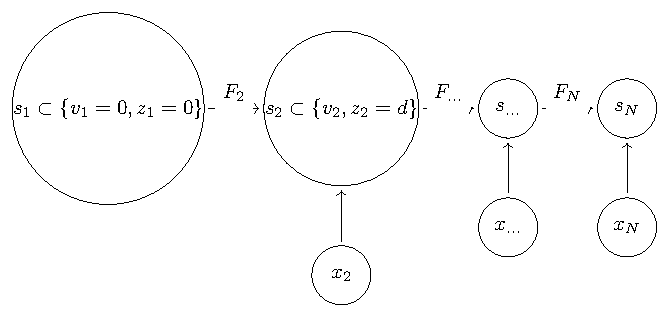
\includegraphics[width = 0.8\textwidth]{figures/graph.pdf}
		\caption{}
		\label{fig:1}
	\end{figure}
	Suppose the Robot is given all historical data, then the expected cost can be written
	\begin{equation}
		\mathbb{E}_{S|X}[C(U(X),S|s_1,\{x\}_{2:N},I)] = \int ds (U(x_N)-s)^2p(s|s_1,\{x\}_{2:N},I).
	\end{equation}
	The optimal decision is defined by
	\begin{equation}
		\frac{d}{dU(X)}\bigg(\mathbb{E}_{S|X}[C(U(X),S|s_1,\{x\}_{2:N},I)]\bigg)\bigg|_{U(x_N)=U^*(x_N)} = 0
	\end{equation}
	leading to (\thref{theorem:expectation_decision_rule})
	\begin{equation}
		U^*(x_N) = \mathbb{E}[S_{N}|s_1,\{x\}_{2:N},I].
		\label{eq:dr}
	\end{equation}
	The inutitive interpretation of \EQref{eq:dr} is that the optimal decision of the Robot is to estimate the position that it expects Nature to have chosen. Now
	\begin{equation}
		\mathbb{E}[S_{N}|s_1,\{x\}_{2:N},I] = \int ds_{N} s_N p(s_N|s_1,\{x\}_{2:N},I).
		\label{eq:a5}
	\end{equation}
	Assume that
	\begin{equation}
		\begin{split}
			p(s_i|s_{i-1},I) &= N(s_i|\mu_i = F_is_{i-1}+b_i,\Sigma_i = Q_i),\\
			p(x_i|s_{i},I) &= N(x_i|\mu_i = H_is_{i}+d_i,\Sigma_i = R_i)
		\end{split}
		\label{eq:a2}
	\end{equation}
	Hence, $p(s_N|s_1,\{x\}_{2:N},I)$ must be reformulated such that the above can be utilized. 
	Now
	\begin{equation}
		\begin{split}
			p(s_N|s_1,\{x\}_{2:N},I) &= \frac{p(x_{N}|s_N,s_1,\{x\}_{2:N-1},I)p(s_N|s_1,\{x\}_{2:N-1},I)}{p(x_{N}|s_1,\{x\}_{2:N-1},I)}\\
			&= \frac{p(x_{N}|s_N,I)p(s_N|s_1,\{x\}_{2:N-1},I)}{p(x_{N}|s_1,\{x\}_{2:N-1},I)}\\
		\end{split}
		\label{eq:a3}
	\end{equation}
	where
	\begin{equation}
		\begin{split}
			p(s_N|s_1,\{x\}_{2:N-1},I) &= \int ds_{N-1}p(s_N,s_{N-1}|s_1,\{x\}_{2:N-1},I)\\
			&= \int ds_{N-1}p(s_N|s_{N-1})p(s_{N-1}|s_1,\{x\}_{2:N-1},I)\\
			&=N(s_{N}|\mu_{N|N-1},\Sigma_{N|N-1})
		\end{split}
		\label{eq:a1}
	\end{equation}
	where 
	\begin{equation}
		\begin{split}
			\mu_{N|N-1} &= F_{N}\mu_{N-1}+b_N\\
			\Sigma_{N|N-1} &= F_{N}\Sigma_{N-1}F_{N}^T+Q_{N}\\
		\end{split}
	\end{equation}
	Using \EQref{eq:a1} and \EQref{eq:a2} in \EQref{eq:a3} then yields~\citep{murphy2023probabilistic}
	\begin{equation}
		p(s_N|s_1,\{x\}_{2:N},I) = N(s_N|\mu_{N},\Sigma_N)
		\label{eq:a4}
	\end{equation}
	where
	\begin{equation}
		\begin{split}
			\mu_{N} &= \mu_{N|N-1}+K_N(x_N-\hat{x}_N),\\
			\Sigma_{N} &= \Sigma_{N|N-1}-K_NS_NK_N^T,\\
			K_N & = \Sigma_{N|N-1}H_N^TS_N^{-1},\\
			\hat{x}_N&= H_N\mu_{N|N-1}+d_N,\\
			S_N & = H_N\Sigma_{N|N-1}H_N^T+R_N\\
		\end{split}
	\end{equation}
	Combining \EQref{eq:a4} with \EQref{eq:a5} then yields the optimal decision for the Robot
	\begin{equation}
		\mathbb{E}[S_{N}|s_1,\{x\}_{2:N},I] = \mu_{N}.
	\end{equation}
	
\end{example}

\begin{example}
	Consider a Robot moving in one dimension. Every time interval $\Delta t$, the Robot will sample a wheel counter and an accelerometer. The wheel counter will be incremented every distance $d$. The Robot is interested in knowing its position and velocity. Expand the position viz
	\begin{equation}
		z(t+\Delta t)=z(t)+\Delta t \frac{dz(t)}{dt}+\frac{1}{2}(\Delta t)^2\frac{d^2z(t)}{dt^2}+\mathcal{O}(\Delta t^3)
	\end{equation}
	which discretize to
	\begin{equation}
		z_k\simeq z_{k-1}+\Delta t v_{k-1}+\frac{1}{2}(\Delta t)^2a_{k-1},
	\end{equation}
	where $\Delta t = \text{const}$ and
	\begin{equation}
		\begin{split}
			v_k &\simeq v_{k-1}+\Delta t a_{k-1},\\
			a_k &\simeq a_{k-1},
		\end{split}
	\end{equation}
	This means
	\begin{equation}
		\begin{split}
			s_k &= \begin{pmatrix}
				z_k\\ v_{k} \\ a_k\\
			\end{pmatrix}\\
			& \simeq \underbrace{\begin{pmatrix}
					1 & \Delta t & \frac{1}{2}\Delta t^2  \\
					0 & 1 & \Delta t  \\
					0 & 0 & 1  \\
			\end{pmatrix}}_{=F_k}\begin{pmatrix}
				z_{k-1}\\ v_{k-1} \\ a_{k-1}\\
			\end{pmatrix}
		\end{split}
	\end{equation}
	where $b_k=\emptyset$ for simplicity. Now take
	\begin{equation}
		\begin{split}
			x_k &= \begin{pmatrix}
				c_k \\ a_k
			\end{pmatrix}\\
			&= \underbrace{\begin{pmatrix}
					d^{-1} & 0 & 0\\
					0 & 0 & 1 
			\end{pmatrix}}_{=H_k}\begin{pmatrix}
				z_{k-1}\\ v_{k-1} \\ a_{k-1}\\
			\end{pmatrix}+r_k
		\end{split}
	\end{equation}
	where $r_k \sim N(0,R_k)$ with 
	\begin{equation}
		R_k = \begin{pmatrix}
			\sigma_z^2 & \sigma_z\sigma_a\\
			\sigma_z\sigma_a & \sigma_a^2 \\
		\end{pmatrix},
	\end{equation}
	where $\sigma_z$ and $\sigma_a$ are estimated from observations. The process noise can be determined viz~\href{https://github.com/rlabbe/Kalman-and-Bayesian-Filters-in-Python/blob/master/07-Kalman-Filter-Math.ipynb}{Kalman link}
	\begin{equation}
		Q_k = \begin{pmatrix}
			\frac{\Delta t^4}{4} & \frac{\Delta t^3}{2} & \frac{\Delta t^2}{2}\\
			\frac{\Delta t^3}{2} & \Delta t^2 & \Delta t\\
			\frac{\Delta t^2}{2} & \Delta t & 1\\
		\end{pmatrix}\sigma^2,
	\end{equation}
	where $\sigma \sim \Delta a$.
\end{example}


\subsection{Bayesian Classification}
\label{chp:baycl}
Classification is the discrete version of regression, meaning it involves the Robot building a model, $f: \Omega_W\times \Omega_X\mapsto[0,1]$, with associated parameters $w\in \Omega_W$, that estimates Nature's actions $S$ based on observed data $X$. As opposed to regression, the random variable $S$ is now discrete and the function is identified with the probability of each action
\begin{equation}
	p(S = s|x,w,I)= f_{S = s}(w,x),
	\label{f_dist2}
\end{equation}
with
\begin{equation}
	\sum_{s\in\mathbb{S}} p(S = s|x,w,I) = 1.
\end{equation}
In this case, the Robot's action space is equal to Natures action space, with the possible addition of a reject option, $\Omega_U=\Omega_S\cup \text{"Reject"}$. To reivew this subject the Robot will be considered to be penalized equally in case of a classification error, which corresponds to the $0-1$ cost function, with the addition of a reject option at cost $\lambda$. This means
\begin{equation}
	C(U(x),s) = 1- \delta_{U(x),s}+(\lambda-1)\delta_{U(x),\text{"Reject"}}.
\end{equation}
The optimal decision rule for the robot can the be written
\begin{equation}
	\begin{split}
		U^*(x) & = \arg\min_{U(x)}\mathbb{E}[C(U(X), S)|x,D,I]\\
		&= \arg\min_{U(x)}\bigg(\sum_{s}C(U(x),s)p(S = s|x,D,I)\\
		&\qquad\qquad\qquad+(\lambda-1)\delta_{U(x),\text{"Reject"}}\bigg)\\
		& = \arg\min_{U(x)}\bigg(1- p(S=U(x)|x,D,I)\\
		&\qquad\qquad\qquad+(\lambda-1)\delta_{U(x),\text{"Reject"}}\bigg).
	\end{split}
	\label{eq:expected_cost1}
\end{equation}
In absence of the reject option, the optimal decision rule is to pick the MAP, similar to \thref{theorem:MAP}. Using \EQref{f_dist2} and marginalizing over $w$
\begin{equation}
	\begin{split}
		p(S= U(x)|x,D,I) &= \int p(S = U(x),w|x,D,I) dw \\
		& = \int p(S = U(x)|x,w,D,I)  p(w|x,D,I)dw \\
		& = \int p(S = U(x)|x,w,I)  p(w|D,I)dw \\
		& = \int f_{S = U(x)}(w,x)  p(w|D,I)dw \\
		& = \mathbb{E}[f_{S = U(x)}(w,x)|D,I],\\
	\end{split}
	\label{eq:q5}
\end{equation}
where for the second to last equality it has been assumed that
\begin{equation}
	p(S = U(x)|w,x,D,I) = p(S = U(x)|w,x,I)
\end{equation}
since by definition $f$ (see \EQref{f_dist2}) produce a $1-1$ map of the input $x$ and $p(w|x,D,I) = p(w|D,I)$ from \axref{ax:observation_relevance}. From Bayes theorem
\begin{equation}
	p(w|D,I) =\frac{p(D_s|D_x,w,I)p(w|D_x,I)}{p(D_s|D_x,I)},
\end{equation}
where from \axref{ax:observation_relevance} $p(w|D_x,I) = p(w|I)$. Assuming the distribution over $w$ is normally distributed with zero mean and a precision described by a hyperparameter, $\lambda$, 
\begin{equation}
	p(w|I) = \int p(w|\lambda,I)p(\lambda|I)d\lambda.
\end{equation}
where $p(w|\lambda,I)p(\lambda|I)$ is given by \EQref{eq:prior}. Assuming the past actions of Nature are independent and identically distributed, the likelihood can be written~\citep{Fischer1999} 
\begin{equation}
	\begin{split}
		p(D_s|D_x,w,I) &=\prod_{i=1}^{n}p(S = s_i|X = x_i,w,I)\\
		&=\prod_{i=1}^{n}f_{s_i}(w,x_i)\\
	\end{split}.
	\label{lik}
\end{equation}
At this point \EQref{eq:expected_cost1} is fully specified and can be approximated by HMC similarly to the regression case. In this case, the model can be represented by the Hamiltonian 
\begin{equation}
	H \equiv  \sum_{q}\sum_{l}\frac{p_{l}^2}{2m_{l}}-\ln(p(w,\lambda|D,I))+const
	\label{ham3}
\end{equation}
where
\begin{equation}
	p(w|D,I) = \int d\lambda p(w,\lambda|D,I).
\end{equation}
Using \EQref{eq:q5}-\EQref{lik} in equation \eqref{ham3} yields the Hamiltonian
\begin{equation}
	\begin{split}
		H&=\sum_{q=1}^{\tilde{n}}\sum_{l=1}^{n_q}\frac{p_{l}^2}{2m_{l}}-\sum_{i=1}^{n}\ln(f_{s_i}(w,x_i))+\text{const}\\
		&\quad+\sum_{q=1}^{\tilde{n}}\bigg(\ln(\Gamma(\alpha_q))-\alpha_q\ln(\beta_q)+(1-\alpha_q)\ln(\lambda_q)+\beta_q\lambda_q\\
		&\qquad \qquad+\frac{n_q}{2}(\ln(2\pi)-\ln(\lambda_q))+\frac{\lambda_q}{2}\sum_{l=1}^{n_q}w_l^2\bigg)\\
	\end{split}.
	\label{ham2}
\end{equation}
Sampling \EQref{ham2} yields a set of coefficients which can be used to compute $\mathbb{E}[f_s(w,x)|D,I]$ which in turn (see \EQref{eq:q5}) can be used to compute $U^*(x)$.


\begin{example}
	\index{Example: Bayesian decision theory}
	\emph{Consider a discrete action space with an observation $X=x$ and available data $D$. Picking a class corresponds to an action, so classification can be viewed as a game against nature, where nature has picked the true class and the robot has to pick a class as well. Suppose there are only two classes and the cost function is defined by the matrix}
	\begin{center}
		\begin{tabular}{ c  c  c  c }
			&& $S$& \\
			&& $s_1$ & $s_2$  \\
			\cline{3-4}
			$U(x)$ & $u_1$& \multicolumn{1}{|l}{$0$} &\multicolumn{1}{l|}{$\lambda_{12}$}  \\
			& $u_2$& \multicolumn{1}{|l}{$\lambda_{21}$} & \multicolumn{1}{l|}{0} \\
			\cline{3-4}
		\end{tabular}
	\end{center}
	\begin{enumerate}
		\item \emph{Show that the decision $u$ that minimizes the expected loss is equivalent to setting a probability threshold $k$ and predicting $U(x)=u_1$ if $p(S=s_2|x,D,I) < k$ and $U(x)=u_2$ if $p(S=s_2|x,D,I)\geq k$. What is $k$ as a function of $\lambda_{12}$ and $\lambda_{21}$?}\newline
		
		The conditional expected cost
		\begin{equation}
			\begin{split}
				\mathbb{E}_{S|X}[C(u, S)|x,D,I] & = \sum_sC(u,S=s)p(S=s|x,D,I)\\
				& = C(u,S=s_1)p(S=s_1|x,D,I)\\
				& \quad+C(u,S=s_2)p(S=s_2|x,D,I)\\
			\end{split}
		\end{equation}
		For the different possible actions
		\begin{equation}
			\begin{split}
				\mathbb{E}_{S|X}[C(u_1, S)|x,D,I] &= \lambda_{12}p(S=s_2|x,D,I),\\
				\mathbb{E}_{S|X}[C(u_2, S)|x,D,I] &= \lambda_{21}p(S=s_1|x,D,I),\\
			\end{split}
		\end{equation}
		$U(x)=u_1$ iff
		\begin{equation}
			\mathbb{E}_{S|X}[C(u_1,S)|x,D,I]<\mathbb{E}_{S|X}[C(u_1,S)|x,D,I])
		\end{equation}
		meaning
		\begin{equation}
			\begin{split}
				\lambda_{12}p(S=s_2|x,D,I)&<\lambda_{21}p(S = s_1|x,D,I)\\
				&=\lambda_{21}(1-p(S =s_2|x,D,I))
			\end{split}
		\end{equation}
		meaning $U(x) = u_1$ iff
		\begin{equation}
			p(S=s_2|x,D,I)<\frac{\lambda_{21}}{\lambda_{12}+\lambda_{21}}=k
		\end{equation}
		
		
		\item \emph{Show a loss matrix where the threshold is $0.1$.}\newline
		
		$k = \frac{1}{21}=\frac{\lambda_{21}}{\lambda_{12}+\lambda_{21}} \Rightarrow \lambda_{12}=9\lambda_{21}$ yielding the loss matrix
		
		\begin{center}
			\begin{tabular}{ c  c  c  c }
				&& $S$& \\
				&& $s_1$ & $s_2$  \\
				\cline{3-4}
				$U(x)$ & $u_1$& \multicolumn{1}{|l}{$0$} &\multicolumn{1}{l|}{$9\lambda_{21}$}  \\
				& $u_2$& \multicolumn{1}{|l}{$\lambda_{21}$} & \multicolumn{1}{l|}{0} \\
				\cline{3-4}
			\end{tabular}
		\end{center}
		
		You may set $\lambda_{21}=1$ since only the relative magnitude is important in relation to making a decision.
		
	\end{enumerate}
	
	
\end{example}


\begin{example}
	\index{Example: Bayesian decision theory}
	\emph{In many classification problems one has the option of assigning $x$ to class $k\in K$ or, if the robot is too uncertain, choosing a reject option. If the cost for rejection is less than the cost of falsely classifying the object, it may be the optimal action. Define the cost function as follows}
	\begin{equation}
		C(u,s)=\begin{cases}
			0 & \text{if correct classification ($u=s$)}\\
			\lambda_r & \text{if reject option $u=$ reject}\\
			\lambda_s & \text{if wrong classification ($u\neq s$)}\\
		\end{cases}.
	\end{equation}
	
	\begin{enumerate}
		\item \emph{Show that the minimum cost is obtained if the robot decides on class $u$ if $p(S=u|x,D,I)\geq p(S\neq u|x,D,I)$ and if $p(S=u|x,D,I)\geq 1-\frac{\lambda_r}{\lambda_s}$.}\newline
		
		The conditional expected cost if the robot does not pick the reject option, meaning $u\in \mathbb{U}\setminus\text{reject}$
		\begin{equation}
			\begin{split}
				\mathbb{E}_{S|X}[C(u, S)|x,D,I] & = \sum_s C(u,S=s)p(S=s|x,D,I)\\
				&= \sum_{s\neq u}\lambda_sp(S=s|x,D,I)\\
				&= \lambda_s(1-p(S=u|x,D,I))
			\end{split}
			\label{eq:cost1}
		\end{equation}
		where for the second equality it has been used that the cost of a correct classification is $0$, so the case of $S=u$ does not enter the sum. For the third equality it has been used that summing over all but $S=u$ is equal to $1-p(S=u|x,D,I)$. The larger $p(S=u|x,D,I)$, the smaller loss (for $\lambda_s>0$), meaning the loss is minimized for the largest probability. The conditional expected loss if the robot picks the reject option
		\begin{equation}
			\begin{split}
				\mathbb{E}_{S|X}[C(\text{reject}, S)|x,D,I]&= \lambda_r\sum_sp(S=s|x,D,I)\\
				&=\lambda_r.
			\end{split}
			\label{eq:cost2}
		\end{equation}
		Equation \eqref{eq:cost1} show picking $\arg\max_{u\in \mathbb{U}\setminus \text{reject}} p(S=u|x,D,I)$ is the best option among classes $u\neq \text{reject}$. To be the best option overall, it also needs to have lower cost than the reject option. Using equations \eqref{eq:cost1} and \eqref{eq:cost2} yields
		\begin{equation}
			(1-p(S=u|x,D,I))\lambda_s< \lambda_r
		\end{equation}
		meaning
		\begin{equation}
			p(S=u|x,D,I)\geq 1-\frac{\lambda_r}{\lambda_s}.
		\end{equation}
		
		\item \emph{Describe qualitatively what happens as $\frac{\lambda_r}{\lambda_s}$ is increased from $0$ to $1$.}\newline
		
		$\frac{\lambda_r}{\lambda_s}=0$ means rejection is rated as a successful classification -- i.e. no cost associated -- and this become the best option (rejection that is) unless $p(y=j|x)=1$, corresponding to knowing the correct class with absolute certainty. In other words; in this limit rejection is best unless the robot is certain of the correct class. $\frac{\lambda_r}{\lambda_s}=1$ means rejection is rated a misclassification -- i.e. $\lambda_r=\lambda_s$ -- and thus and "automatic cost". Hence, in this case rejection is never chosen. In between the limits, an interpolation of interpretations apply.
	\end{enumerate}
\end{example}



\begin{example}
	\paragraph{Setup:} Consider a farmer who wishes to retire and therefore would like to sell their set of live animals. For simplicity, assume that animals make up a simple group and a given person can either be interested in purchasing an animal or not -- the simplfication consist of not differentiating between different animal types. In order to sell their animals, the farmer needs to contact people with a sale in mind. For simplicity, the contact will be assumed to be via a telephone call only. The farmer can call (or not) with the intent to sell an animal to the recepient of the call. The recepient of the call can (or not) be interesed in purchasing an animal (Natures decision). Let $\Omega_U$ denote the set of the farmers actions and $\Omega_S$ the set of Natures actions, then
	\begin{equation}
		\begin{split}
			\Omega_U &= \{u_1 = \text{call}, u_2 = \text{don't call}\},\\
			\Omega_S &= \{s_1 = \text{interested}, s_2 = \text{not interested}\}.
		\end{split}
	\end{equation}
	A nuisance for the contacted people is associated to the call which is represented by the abstract monetary loss, $\lambda\in \mathbb{R}^+$. The degree to which people are annoyed by a sales call is independent in general and the monetary loss represents the average animosity generated and the associated moneraty loss connected to a worsened reputation. Aside from the nuisance associated with a sales call, there is also a moneraty reward for a successfull sale, $\psi$.	If the farmer cannot sell his animals, he will have them terminated with no associated cost in order not to spend additional time or money on them. Given these assumptions, the cost function can be represented by the matrix
	\begin{center}
		\begin{tabular}{  c  c  c }
			& $s_1=$ Interested & $s_2=$ Not interested  \\
			\cline{2-3}
			 $u_1 =$ Call& \multicolumn{1}{|l}{$\lambda-\psi$} &\multicolumn{1}{l|}{$\lambda$}  \\
			 $u_2=$ Don't call& \multicolumn{1}{|l}{$0$} & \multicolumn{1}{l|}{0} \\
			\cline{2-3}
		\end{tabular}
	\end{center}
	The farmer has available to them observations $X=x$ that contain information regarding the decesion Nature is going to make, $S=s$. The farmer also have a collection of past observations and resulting decisions of Nature, i.e. $D= \{(X=x_1,S=s_1),(X=x_2,S=s_2),\dots (X=x_n,S=s_n)\}= D_s\times D_s$. 
	
	\paragraph{Optimal decision rule:} The optimal decision for the farmer to call the $i$'th person can then be written viz
	\begin{equation}
		U^*(x) = \arg\min_{U(x)} \mathbb{E}_{S|X}[C(U(x), S)|X=x,D,I],
	\end{equation}
	where
	\begin{equation}
		\mathbb{E}_{S|X}[C(U(x), S)|X=x,D,I] = \sum_{s\in \mathbb{S}} C(U(x),s) p(S=s|X=x,D,I).
	\end{equation}
	Writing out the conditional expectation
	\begin{equation}
		\begin{split}
			\mathbb{E}[C(u_1, S)] & = \sum_sC(u_1,s)p(s)\\
			& = C(u_1,s_1)p(s_1|x,D,I) + C(u_1,s_2)p(s_2|x,D,I)\\
			& = (\lambda-\psi)p(s_1|x,D,I) + \lambda_i p(s_2|x,D,I),\\
			\mathbb{E}[C(u_2, S)] & = \sum_sC(u_2,s)p(s|x,D,I)\\
			& = C(u_2,s_1)p(s_1|x,D,I) + C(u_2,s_2)p(s_2|x,D,I),\\
			&=0
		\end{split}
	\end{equation}
	where the notation has been compressed to fit the equations to the page. The optimal decision rule $U^*(x)$ can be implicitly specified as picking $u_1$ (call) iff $\mathbb{E}_{S|X}[C(u_1, S)|x,D,I]<\mathbb{E}_{S|X}[C(u_2, S)|x,D,I]$, corresponding to picking $u_1$ (call) iff
	\begin{equation}
		(\lambda-\psi)p(S= s_1|x,D,I) + \lambda p(S= s_2|x,D,I) <0
	\end{equation}
	Since $p(S= s_1|x,D,I) +p(S= s_2|x,D,I) = 1$
	\begin{equation}
		\frac{\lambda}{\psi} < p(S= s_1|x,D,I)
		\label{eq:decision_rule}
	\end{equation}
	meaning the farmer should call (action $u_1$) iff the probability for the recepient of the call to be interested in at least one animal is larger than the penalty of calling divided by the gain of calling. 
	
	\paragraph{The Probability:} \EQref{eq:decision_rule} implicitly specify the decision rule for the farmer. $\lambda,\psi$ is assumed specified, so only the probability $p(S= s_1|x,D,I)$ remain to be specified. Suppose now a model, $f: \Omega_W\times \Omega_X\mapsto[0,1]$, with associated parameters $w\in \Omega_W$, that estimates Nature's actions $S$ based on observed data $X$ is introduced. Using marginalization and assuming independence 
	\begin{equation}
		\begin{split}
			p(S= s|x,D,I) &= \int p(S= s,w|x,D,I) dw \\
			& = \int p(S= s|x,w,D,I)  p(w|x,D,I)dw \\
			& = \int p(S= s|x,w,I)  p(w|D,I)dw. \\
		\end{split}
		\label{eq:q5}
	\end{equation}
	Combining \EQref{eq:q5} and \EQref{f_dist2}
	\begin{equation}
		\begin{split}
			p(S= s|x,D,I) & = \int f_{S = s}(w,x)  p(w|D,I)dw \\
			& = \mathbb{E}[f_{S = s}(w,x)|D,I].\\
		\end{split}
	\end{equation}
	From Bayes theorem \index{Bayes theorem}
	\begin{equation}
		p(w|D,I) =\frac{p(D_s|D_x,w,I)p(w|D_x,I)}{p(D_s|D_x,I)},
	\end{equation}
	where $p(w|D_x,I) = p(w|I)$. Assuming the distribution over $w$ is normally distributed with zero mean and a precision described by a hyperparameter, $\lambda$, 
	\begin{equation}
		p(w|I) = \int p(w|\lambda,I)p(\lambda|I)d\lambda.
		\label{eq:lambda}
	\end{equation}
	The precision is constructed as a wide gamma distribution so as to approximate an objective prior
	\begin{equation}
		p(w|\lambda,I)p(\lambda|I)
		= \prod_{q=1}^{\tilde{n}} \frac{\lambda_q^\frac{n_q}{2}}{(2\pi)^\frac{n_q}{2}}e^{-\frac{\lambda_q}{2}\sum_{l=1}^{n_q}w_l^2}\frac{\beta_q^{\alpha_q}}{\Gamma(\alpha_q)}\lambda_q^{\alpha_q-1}e^{-\beta_q \lambda_q}
		\label{eq:prior}
	\end{equation}
	Assuming the past actions of Nature are independent and identically distributed, the likelihood can be written 
	\begin{equation}
		\begin{split}
			p(D_s|D_x,w,I) &=\prod_{i=1}^{n}p(S = s_i|X = x_i,w,I)\\
			&=\prod_{i=1}^{n}f_{s_i}(w,x_i).\\
		\end{split}
		\label{lik}
	\end{equation}
	Aside from the specification of the model $f$, $p(S= s|x,D,I)$ is at this point fully specified and can be approximated by HMC similarly to the regression case. In this case, the model can be represented by the Hamiltonian 
	\begin{equation}
		H \equiv  \sum_{q}\sum_{l}\frac{p_{l}^2}{2m_{l}}-\ln(p(w,\lambda|D,I))+const
		\label{ham3}
	\end{equation}
	where
	\begin{equation}
		p(w|D,I) = \int d\lambda p(w,\lambda|D,I).
	\end{equation}
	Using \EQref{eq:q5}-\EQref{lik} in \EQref{ham3} yields the Hamiltonian
	\begin{equation}
		\begin{split}
			H&=\sum_{q=1}^{\tilde{n}}\sum_{l=1}^{n_q}\frac{p_{l}^2}{2m_{l}}-\sum_{i=1}^{n}\ln(f_{s_i}(w,x_i))+\text{const}\\
			&\quad+\sum_{q=1}^{\tilde{n}}\bigg(\ln(\Gamma(\alpha_q))-\alpha_q\ln(\beta_q)+(1-\alpha_q)\ln(\lambda_q)+\beta_q\lambda_q\\
			&\qquad \qquad+\frac{n_q}{2}(\ln(2\pi)-\ln(\lambda_q))+\frac{\lambda_q}{2}\sum_{l=1}^{n_q}w_l^2\bigg)\\
		\end{split}.
		\label{ham2}
	\end{equation}
	
	\paragraph{Simple model:} Let
	\begin{equation}
		f_{S = s}(w,x_i) = \frac{e^{b_s+\sum_{q}a_{sq}x_{iq}}}{\sum_{k\in \mathbb{S}}e^{b_k+\sum_{q}a_{kq}x_{iq}}},
		\label{eq:f1}
	\end{equation}
	where $w = \{b,a\}$.
	
	\paragraph{Manual HMC:}	The Hamiltonian is given by
	\begin{equation}
		\begin{split}
			H&=\sum_{q=1}^{2}\sum_{l=1}^{2}\frac{p_{ql}^2}{2m_{ql}}-\sum_{i=1}^{n}\ln(f_{s_i}(w,x_i))\\
			&\quad+\ln(\Gamma(\alpha_a))-\alpha_a\ln(\beta_a)+(1-\alpha_a)\ln(\lambda_a)+\beta_a\lambda_a\\
			&\qquad \qquad+\frac{1}{2}(\ln(2\pi)-\ln(\lambda_a))+\frac{\lambda_a}{2}\sum_{j,q}a_{jq}^2\\
			&\quad+\ln(\Gamma(\alpha_b))-\alpha_b\ln(\beta_b)+(1-\alpha_b)\ln(\lambda_b)+\beta_b\lambda_b\\
			&\qquad \qquad+\frac{1}{2}(\ln(2\pi)-\ln(\lambda_b))+\frac{\lambda_b}{2}\sum_{j}b_j^2\\
		\end{split}
	\end{equation}
	$\lambda_j$ is positive definite. In order to uphold this numerically, let $\lambda_j = e^{\tau_j}$. When making this transformation, the integration measure of \EQref{eq:lambda} has to be transformed as well. This proceeds viz
	\begin{equation}
		d\lambda_j = \lambda_jd\tau_j,
	\end{equation}
	meaning effectively $\lambda_j$ is multiplied on $p(w,\lambda|D,I)$ such that $H \rightarrow H-\ln(\lambda_j)$. This means
	\begin{equation}
		(1-\alpha_j)\ln(\lambda_j)\in H \Rightarrow -\alpha_j \ln(\lambda_j).
	\end{equation}
	Additionally, it is convenient to pick out the $s_i$ via a one-hot target vector such that
	\begin{equation}
		\begin{split}
			H&=\sum_{q=1}^{2}\sum_{l=1}^{2}\frac{p_{ql}^2}{2m_{ql}}-\sum_{j\in \mathbb{S}}\sum_{i=1}^{n}s_{ij}\ln(f_{j}(w,x_i))\\
			&\quad+\ln(\Gamma(\alpha_a))-\alpha_a\ln(\beta_a)-\alpha_a\tau_a+\beta_ae^{\tau_a}\\
			&\qquad \qquad+\frac{1}{2}(\ln(2\pi)-\tau_a)+\frac{e^{\tau_a}}{2}\sum_{j,q}a_{jq}^2\\
			&\quad+\ln(\Gamma(\alpha_b))-\alpha_b\ln(\beta_b)-\alpha_b\tau_b+\beta_be^{\tau_b}\\
			&\qquad \qquad+\frac{1}{2}(\ln(2\pi)-\tau_b)+\frac{e^{\tau_b}}{2}\sum_{j}b_j^2\\
		\end{split}
	\end{equation}
	
	The derivatives are needed for the HMC algorithm
	\begin{equation}
		\frac{\partial H}{\partial a_{ml}} = -\sum_{i,j}\frac{s_{ij}}{f_{ij}}\frac{\partial f_{ij}}{\partial a_{ml}}+e^{\tau_a}a_{ml},\\
	\end{equation}
	\begin{equation}
		\begin{split}
			\frac{\partial f_{ij}}{\partial a_{ml}} & = \frac{e^{b_j+\sum_{q_1}a_{jq_1}x_{iq_1}}}{\sum_{k\in \mathbb{S}}e^{b_k+\sum_{q_2}a_{kq_2}x_{iq_2}}}\sum_{q_3}\delta_{jm}\delta_{q_3l}x_{iq_3}\\
			&\qquad-\frac{e^{b_j+\sum_{q_4}a_{jq_4}x_{iq_4}}}{(\sum_{k\in \mathbb{S}}e^{b_k+\sum_{q_5}a_{kq_5}x_{iq_5}})^2}\sum_{k'\in \mathbb{S}}e^{b_{k'}+\sum_{q_6}a_{k'q_6}x_{iq_6}}\sum_{q_7}\delta_{k'm}\delta_{q_7l}x_{iq_7}\\
			& = f_{ij}\delta_{jm}x_{il}- f_{ij}f_{im}x_{il}
		\end{split}
	\end{equation}
	where it has been used that
	\begin{equation}
		\frac{\partial a_{jq_3}}{\partial a_{ml}} = \delta_{jm}\delta_{q_3l}
	\end{equation}
	
	\begin{equation}
		\begin{split}
			\frac{\partial H}{\partial a_{ml}} &= -\sum_{i,j}\frac{s_{ij}}{f_{ij}}(f_{ij}\delta_{jm}x_{il}- f_{ij}f_{im}x_{il})+e^{\tau_a}a_{ml}\\
			& = \sum_ix_{il}(f_{im}-s_{im})+e^{\tau_a}a_m\\
		\end{split}
	\end{equation}
	\begin{equation}
		\frac{\partial H}{\partial b_m} = \sum_i(f_{im}-s_{im})+e^{\tau_b}b_m.
	\end{equation}
	\begin{equation}
		\frac{\partial H}{\partial \tau_m} = -\alpha_m+\beta_me^{\tau_m}-\frac{1}{2}+\frac{e^{\tau_m}}{2}\sum_jm_j^2.
	\end{equation}
	
	The masses for the HMC algorithm can be set by approximating the second order derivatives as fixed. Let
	\begin{equation}
		\begin{split}
			\frac{\partial^2 H}{\partial a_{ml}^2} &= \sum_ix_{il}\frac{\partial f_{im}}{\partial a_{ml}}+e^{\tau_a}\\
			& =\sum_ix_{il}^2f_{im}( 1- f_{im})+e^{\tau_a}\\
		\end{split}
	\end{equation}
	then taking $x_{il}^2\sim 1, f_{im}\sim \frac{1}{2}$ and any parameter $\sim 0$, meaning $e^{\tau_a} \sim 1$ yield the mass approximation
	\begin{equation}
		\begin{split}
			m_{ml}^{(a)} &\sim \frac{\partial^2 H}{\partial a_{ml}^2}\bigg|_{\text{fixed approximation}}\\
			& \sim N\cdot 1^2\cdot \frac{1}{2}(1-\frac{1}{2})+1\\
			&=\frac{N}{4} +1,
		\end{split}
	\end{equation}
	where $N$ is the number of data samples in $D_x$. Similarly
	\begin{equation}
		\begin{split}
			\frac{\partial^2 H}{\partial b_m^2} &= \sum_i\frac{\partial f_{im}}{\partial a_{ml}}+e^{\tau_b}\\
			& =\sum_if_{im}( 1- f_{im})+e^{\tau_b},
		\end{split}
	\end{equation}
	meaning (since $x_{il}^2\sim 1$)
	\begin{equation}
		\begin{split}
			m_{ml}^{(a)} &\sim \frac{\partial^2 H}{\partial b_{m}^2}\bigg|_{\text{fixed approximation}}\\
			& m_{ml}^{(b)}.
		\end{split}
	\end{equation}
	The precision parameter
	\begin{equation}
		\frac{\partial^2 H}{\partial \tau_q^2} = \beta_qe^{\tau_q}+\frac{e^{\tau_q}}{2}\sum_jq_j^2.
	\end{equation}
	Take $\beta_q = 3$, then
	\begin{equation}
		\begin{split}
			m_{q}^{(\tau)} &\sim \frac{\partial^2 H}{\partial \tau_{q}^2}\bigg|_{\text{fixed approximation}}\\
			&\sim 3.
		\end{split}
	\end{equation}
	
	
	
	
	\paragraph{Data:} Take $x=(\text{area},\text{number of animals})^T$ and $s=$ 2d one-hot vector, with $\dim(D)=1000$. $D$ is split into two sets $D^{(\text{training})}$ and $D^{(\text{test})}$, with $\dim(D^{(\text{training})})=\gamma\dim(D)$ and $\dim(D^{(\text{test})})=(1-\gamma)\dim(D)$ and $\gamma=0.6$. $D^{(\text{training})}$ will be used to train the model and $D^{(\text{test})}$ to evaluate the quality of the trained model. The underlying truth of Nature (unbeknownst to the model) is that an animal will be purchased iff
	\begin{equation}
		\text{total area}- 3.2\cdot\text{number of animals}\geq 3.2.
		\label{eq:nature}
	\end{equation}
	
	\paragraph{Training:} Using $D^{(\text{training})}$ as input, the algorithms the algorithms are trained for $2000$ iterations. The first $500$ iterations are taken as burn in to be conservative. The coefficients, $w$, for iterations $[500,2000]$ are used to make a model prediction viz
	\begin{equation}
		p(S= s|x,D,I)=\frac{1}{1500}\sum_{i=500}^{2000}f(w_i,x)
	\end{equation}
	The accuracy of the modeled probabilities can be gauged by considering the case where $\psi=2\lambda$ such that the decision rule (\EQref{eq:decision_rule}) becomes
	\begin{equation}
		\frac{1}{2} < p(S= s_1|x,D,I),
		\label{eq:decision_rule2}
	\end{equation}
	and the classification is driven by the probabilities alone. 
	
	
	\paragraph{PyMC HMC Algorithm:} PyMC is a probabilistic programming library for Python that allows users to build Bayesian models with a Python API and fit them using Markov Chain Monte Carlo methods \href{https://www.pymc.io/welcome.html}{PyMC link}. Using this API it is possible to create, train and test a PyMC-equivalent of the model described in the previous sections. The general approach to building a model using PyMC consists of stating the data generating process, specifying a likelihood, and related prior distributions for any parameters involved. While modeling the data generating process and framing the statistical problem correctly are never completely trivial and require some effort from the user it is rather straight forward to perform the Markov Chain Monte Carlo sampling with PyMC. The user do not need to do any calculations related to the Hamiltonian Monte Carlo method nor do they need to specifically handle any integrals. In addition, there is a range of predefined probability distributions both discrete and continuous readily available in the library such as the Gamma (figure \ref{fig:gamma}) and Normal distribution used for modeling the priors.
	\begin{figure}[H]
		\centering
		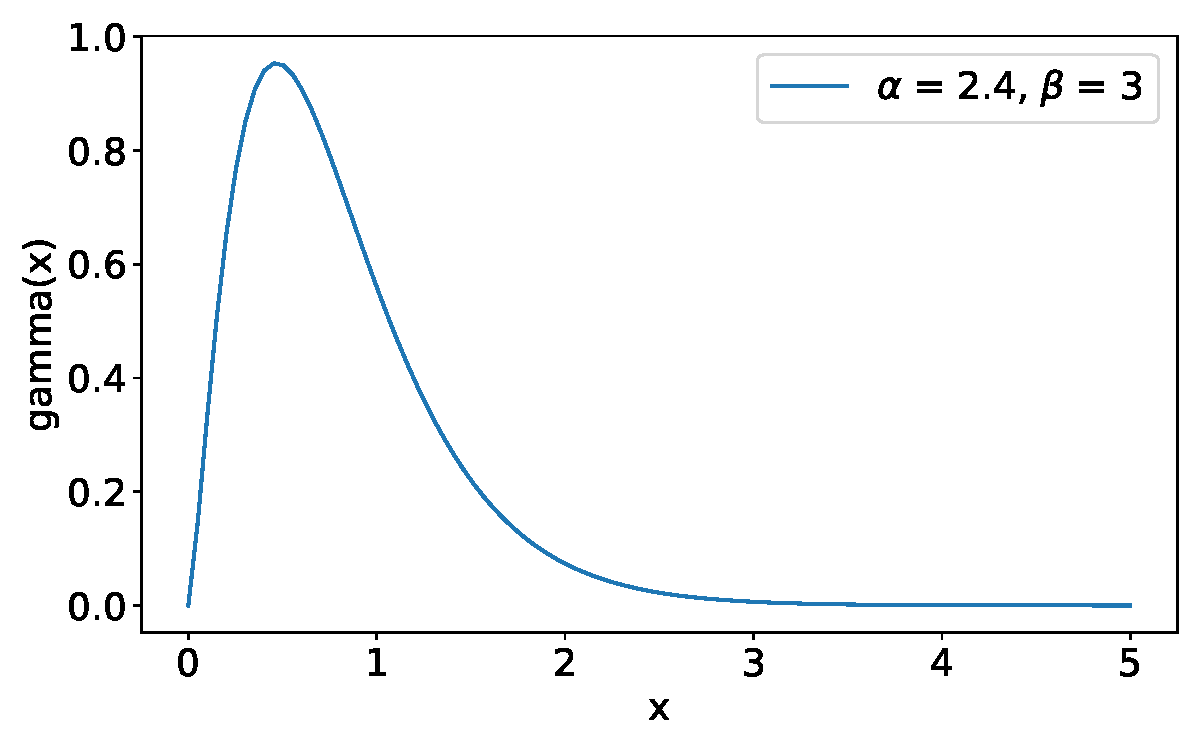
\includegraphics[width = 1\textwidth]{figures/gamma_dist.pdf}
		\caption{Plot of Gamma probability distribution used as priors for the precision parameters in Normal distributions.}
		\label{fig:gamma}
	\end{figure}
	The python code in \algref{algo:pymc_model} shows how the simple model can be declared using PyMC. All models in PyMC are declared using a "with pm.Model() as modelname"-statement, where pm is the abbreviated form of the PyMC package. Within this statement at range of random variables, data and their relations can be declared. The syntax for declaring a random variable by its probability distribution (such as pm.Normal) is to pass a name for the random variable as a string for the first argument. The rest of the arguments are typically values for the parameters specific to the distribution. PyMC random variables can often be used for stating parameters in other random variables forming a hierarchy of distributions as is the case for the precision variables used to model the variance for the normally distributed parameters a and b (see \EQref{eq:f1}) with zero mean. In the code example, these parameters are then combined deterministically with $D_x$ to constitute the data generating process of the simple model. $D_x$ is declared as a PyMC mutable object so that it will be possible later to change the values to generate predictions. As a last step the likelihood is declared. In PyMC this is the step where the relationship between the observed conditional ($D_s$) data and parameters is stated. As the output is the probabilities for the two classes a Multinomial distribution with the number of independent trials (n) equal to 1 is used as the likelihood. 
	
	\begin{algorithm}[H]
		\caption{PyMC Python Code}
		\begin{python}
			import pymc as pm
			import numpy as np
			with pm.Model() as classifier_model:
			covars = pm.MutableData('covars',data_x_training) 
			# Priors for precision
			precision_a = pm.Gamma('precision_a', alpha=2.4, beta=3)
			precision_b = pm.Gamma('precision_b', alpha=2.4, beta=3)
			# Priors for parameters
			param_a = pm.Normal('param_a', 
			0, 
			sigma=1/np.sqrt(precision_a),
			shape=(2,2))
			param_b = pm.Normal('param_b', 
			0, 
			sigma=1/np.sqrt(precision_b),
			shape=(2,))
			# Data generating process
			T = pm.Deterministic('T', pm.Math.exp(param_b + pm.math.dot(covars, param_a.T)))
			class_conditional_probability = pm.Deterministic('class_conditional_probability', T/T.sum(axis=1, keepdims=True))
			# Likelihood
			obs = pm.Multinomial('obs', n=1, p=class_conditional_probability, observed=data_s_training, shape=class_conditional_probability.shape)
		\end{python}
		\label{algo:pymc_model}
	\end{algorithm}
	
	
	After declaring the model it is possible to sample the posterior by calling the pm.sample() method. Burn-in can be controlled by setting the tune argument. The draw argument determines how many samples are being drawn while a number of chains can be run in parallel by setting the chains and cores (computational) arguments. 	
	\begin{algorithm}[H]
		\label{algo:posteriro}
		\caption{PyMC Posterior Python Code}
		\begin{python}
			with classifier_model:
			posterior = pm.sample(tune=512, draws=1024, chains=4, cores=4)
		\end{python}  
	\end{algorithm}
	
	Using the result of drawing samples from the distribution of model parameters (posterior) it is possible to draw from the posterior predictive distribution using the pm.sample\_posterior\_predictive() method. Without changing the input data this is equivalent to obtaining the result of applying the trained model on $D_x^{(\text{training})}$. By changing the input data to $D_x^{(\text{test})}$ using the pm.set\_data() method it is possible to obtain the posterior predictive distribution.
	
	\begin{algorithm}[H]
		\label{algo:posteriro_predictive}
		\caption{PyMC Posterior Python Code}
		\begin{python}
			with classifier_model:
			posterior_predictive = pm.sample_posterior_predictive(posterior)
			pm.set_data({'covars': data_x_test})
			posterior_predictive_test = pm.sample_posterior_predictive(posterior)
		\end{python}
	\end{algorithm}
	
	Using \EQref{eq:decision_rule2} for $D^{(\text{training})}$, the PyMC model correctly classify $598$ of $600$ data points. For $D^{(\text{test})}$, the model correctly classify $398$.
	
	\paragraph{Results: } The HMC algorithm have parameters "step\_scale" and "number\_of\_steps\_scale", which adjust the overall scale of the step lengths and number of steps in pase space. Ideally, the distance between points should be large, so that step scale should be small (what the step length is divided by should be small) and the number of steps should be large. Numerical stability only exist for step\_scale $\gtrsim 5$ (given accurate mass estimation) and thus only the number of steps remain as a variable to tune. In this study step\_scale $=10$ and number\_of\_steps\_scale $=1500$, where the latter is limited by reasonable computation time (to match approximately the pymc computation time). Given these parameters, the manual HMC algorithm misclassify a single training data point
	\begin{equation}
		x^{(\text{training})}_{\text{misclassified 1}} = \begin{pmatrix}
			3.21798365\\ 0\\
		\end{pmatrix}
		\label{eq:misclassified1_training}
	\end{equation}
	and two test data points
	\begin{equation}
		x^{(\text{test})}_{\text{misclassified 1}} = \begin{pmatrix}
			6.40501793\\ 1\\
		\end{pmatrix}, \quad x^{(\text{test})}_{\text{misclassified 2}} = \begin{pmatrix}
			9.60627827\\ 2\\
		\end{pmatrix}.
		\label{eq:misclassified1_test}
	\end{equation}
	With \EQref{eq:nature} in mind, it is clear that the misclassifications of \EQref{eq:misclassified1_training} and \EQref{eq:misclassified1_test} are close to the limit with respect to purchasing an animal.  
	
	
	The PyMC HMC Algorithm obtain misclassify two training data points; \EQref{eq:misclassified1_training} and 
	\begin{equation}
		x^{(\text{training})}_{\text{misclassified 2}} = \begin{pmatrix}
			12.80826256\\ 3\\
		\end{pmatrix}
		\label{eq:misclassified1_training2}
	\end{equation}
	and two test data points (\EQref{eq:misclassified1_test}).
	
	
	\paragraph{Summary and Discussion:} It has been shown how decision theory can be used in conjunction with statistics to make theoretically optimal decisions based on a user specified set of preferences (cost function). Using mock data, a "manual HMC algorithm" written by hand and a standard Python "PyMC HMC algorithm" have been compared. The two yield identical results on test data with the manual model yielding marginally better results on training data. Overall the performace is deemed equivalent both in terms of accuracy and computational speed. The manual HMC algorithm require the user to derive the gradients, write the sampling algorithm in Python and tune the algorith, whereas the latter only require a specification of the model via a standardized PyMC interface. Hence, from a user complexity perspective, the PyMC algorithm has a significant advantage.
\end{example}

\subsection{Making Inference About the Model of Nature}
In some instances, the robot is interested in inference related to the model of Nature. The observation $X=x$ by definition does not have an associated known action of Nature and thus by \axref{ax:observation_relevance} is disregarded in this context. From \EQref{eq:decision_rule3}
\begin{equation}
	U^*(D) = \arg\min_{U(D)} \mathbb{E}_{S|D}[C(U(D), S)|D,I]
	\label{eq:best_decision}
\end{equation}
where $S=s$ is interpreted as an action related to the model of Nature, e.g. Nature picking a given systematic that generates data.


\subsubsection{Selecting the Robot's Model}
\label{sec:model_selection}
Suppose the Robot must choose between two competing models, aiming to select the one that best represents Nature's true model. The two competing models could e.g. be two different functions $f$ in regression or two different probability distribution assignments. In this case the Robot has actions $u_1$ and $u_2$ representing picking either model and Nature has two actions $s_1$ and $s_2$ which represent which model that in truth fit Nature's true model best. From \EQref{eq:best_decision}
\begin{equation}
	\begin{split}
		\mathbb{E}[C(u_1, S)|D,I] =&  \sum_{s = s_1,s_2}C(u_1,s)p(S=s|D,I),\\
		\mathbb{E}[C(u_2, S)|D,I] =&  \sum_{s = s_1,s_2}C(u_2,s)p(S=s|D,I),
	\end{split}
\end{equation}
where in this case $u_i=s_i\quad \forall (u_i,s_i)\in \mathbb{U}\times\mathbb{S}$ but the notational distinction is kept to avoid confusion. Since there is no input $X=x$ in this case, the decision rule $U$ is fixed (i.e. it does not depend on $x$). $U = u_1$ is picked iff $\mathbb{E}[C(U = u_1, S)|D,I]<\mathbb{E}[C(U = u_2, S)|D,I]$, meaning
\begin{equation}
	\frac{p(s_1|D,I)}{p(s_2|D,I)}>\frac{C(u_1,s_2)-C(u_2,s_2)}{C(u_2,s_1)-C(u_1,s_1)}.
\end{equation}
The ratio $\frac{p(s_1|D,I)}{p(s_2|D,I)}$ is referred to as the posterior ratio\index{Posterior ratio}. Using Bayes theorem it can be re-written viz
\begin{equation}
	\begin{split}
		\text{posterior ratio} &= \frac{p(s_1|D,I)}{p(s_2|D,I)}\\
		& = \frac{p(D_s|s_1,D_x,I)p(s_1|I)}{p(D_s|s_2,D_x,I)p(s_2|I)},
	\end{split}
\end{equation}
where for the second equality it has been used that the normalization $p(D|I)$ cancels out between the denominator and nominator and \axref{ax:observation_relevance} has been employed. Given there is no a priori bias towards any model, $p(s_1|I) = p(s_2|I)$
\begin{equation}
	\text{posterior ratio} = \frac{p(D_s|s_1,D_x,I)}{p(D_s|s_2,D_x,I)}.
	\label{eq:bayes_factor}
\end{equation}
$p(D_s|s_1,D_x,I)$ and $p(D_s|s_2,D_x,I)$ can then be expanded via marginalization, the chain rule and Bayes theorem until they can be evaluated either analytically or numerically. \EQref{eq:bayes_factor} is referred to as Bayes factor\index{Bayes factor} and as a rule of thumb

\begin{definition}[Bayes Factor Interpretation Rule of Thumb]
	If the probability of either of two models being the model of Nature is more than 3 times likely than the other, the likelier model is accepted. Otherwise the result does not significantly favor either model.
\end{definition}



\subsubsection{Bayesian Parameter Estimation}
Let $w_j\in \Omega_W$ represent the $j$'th parameter with the associated random variable $W_j$. In case of parameter estimation, the action of Nature is identified with the parameter of interest from the model of Nature's and the Robot's action with the act of estimating the parameters value, meaning
\begin{equation}
	U^*=\arg\min_U\mathbb{E}[C(U, W_j)|D,I],
\end{equation}
with
\begin{equation}
	\mathbb{E}[C(U, W_j)|D,I] = \int dw_j C(U,w_j)p(w_j|D,I).
\end{equation}
At this point, the Robot can select a cost function like in \secref{sec:assing_cost} and proceed by expanding $p(w_j|D,I)$ similarly to \EQref{eq:pa2}. Picking the quadratic cost (\dfref{def:quadratic_cost}) yields 
\begin{equation}
	\begin{split}
		U^* = \mathbb{E}[w_j|D,I]
	\end{split}
	\label{eq:hest2}
\end{equation}
$p(w_j|D,I)$ in \EQref{eq:hest2} can be expanded as shown in \EQref{eq:pa2}.

\begin{example}
	Consider the scenario where two sets of costumers are subjected to two different products, $A$ and $B$. After exposure to the product, the costumer will be asked whether or not they are satisfied and they will be able to answer "yes" or "no" to this. Denote the probability of a costumer liking product $A/B$ by $w_A/w_B$, respectively. In this context, the probabilities $w_A/w_B$ are parameters of Natures model (similar to how the probability is a parameters for a binomial distribution). What will be of interest is the integral of the joint probability distribution where $w_B>w_A$, meaning
	\begin{equation}
		p(w_B > w_A|D,I)= \int_0^1\int_{w_A}^1p(w_A,w_B|D,I)dw_Adw_B.
		\label{e1}
	\end{equation}
	Assuming the costumer sets are independent
	\begin{equation}
		\begin{split}
			p(w_A,w_B|D,I) &= p(w_B|w_A,D,I)p(w_A|D,I)\\
			& = p(w_B|D_A,I)p(w_A|D_A,I),
		\end{split}
	\end{equation}
	with
	\begin{equation}
		p(w_i|D_i,I)=\frac{p(D_i|w_i,I)p(w_i|I)}{p(D_i|I)}.
	\end{equation}
	Assuming a beta prior and a binomial likelihood yields (since the binomial and beta distributions are conjugate)
	\begin{equation}
		p(w_i|D_i,I)=\frac{w_i^{\alpha_i-1}(1-w_i)^{\beta_i-1}}{B(\alpha_i,\beta_i)},
	\end{equation}
	where $\alpha_i\equiv \alpha+s_i$, $\beta_i\equiv \beta+f_i$ and $s_i/f_i$ denotes the successes/failure, respectively, registered in the two sets of costumers. Evaluating \EQref{e1} yields
	\begin{equation}
		p(w_B > w_A|D,I)= \sum_{j=0}^{\alpha_B-1}\frac{B(\alpha_A+j,\beta_A+\beta_B)}{(\beta_B+j)B(1+j,\beta_B)B(\alpha_A,\beta_A)}.
	\end{equation}
	
\end{example}



